\documentclass[11pt]{article}
\usepackage[margin=0.85in]{geometry}
\usepackage{amsmath,amssymb}
\usepackage[utf8]{inputenc}
\usepackage[T1]{fontenc}
\usepackage{mathpazo}
\usepackage[hidelinks]{hyperref}
\usepackage[super]{cite}
\usepackage{tikz}
\usetikzlibrary{decorations.pathreplacing,arrows.meta}
\usepackage{booktabs}
\emergencystretch=3em

\setlength{\parindent}{0pt}
\setlength{\parskip}{4pt plus 1pt minus 1pt}

\title{\vspace{-1.5em}\textbf{One Postulate}}
\author{Emad Mostaque\\[2pt]{\normalsize Intelligent Internet}}
\date{March 2026}

\begin{document}
\maketitle
\thispagestyle{empty}
\vspace{-1.5em}

\begin{abstract}
\noindent Einstein built special relativity on two postulates: no experiment can distinguish one constant-velocity laboratory from another, and light travels at the same speed in every such laboratory. The first is a principle of symmetry. The second is a fact about a particular phenomenon, an observation imported into the foundations. We show this was unnecessary. The symmetry principle alone yields a family of possible universes, labelled by a single number~$\kappa$. The Killing form (a diagnostic built into every set of symmetry rules, introduced by Wilhelm Killing in 1888) sorts them into exactly three kinds: one with no causality, one that cannot unify space and time, and one that achieves both and demands a finite speed that is the same in all frames. Experiment is needed to measure that speed, not to establish its existence. Einstein needed one postulate, not two.
\end{abstract}


\subsection*{The postulate}

Einstein built special relativity on two principles \cite{Einstein1905}. The first is a symmetry requirement:

\textsc{Postulate} (relativity principle, 1905)\textsc{.}\quad\emph{The laws of physics take the same form in all inertial frames.}

\smallskip
An inertial frame is any laboratory moving at constant velocity: a sealed room drifting through space. The postulate says that no experiment performed inside such a room can reveal how fast it is moving, or whether it is moving at all.

For Einstein this was more than a statement about experiments. It was a design principle: the mathematical framework of physics should contain no structure put in by hand. Everything should emerge from the rules themselves. Special relativity came from removing the assumption that all observers agree on which events are simultaneous. General relativity came from removing the assumption that there is a single natural way to label points in spacetime, the four-dimensional union of space and time. Each advance stripped away a background assumption that the previous framework had smuggled in.

The second postulate is different in character. It says that light travels at a finite speed~$c$ that is the same in all inertial frames. This is not a principle of symmetry. It is an observation about a particular physical phenomenon, imported into the foundations. For Einstein, who held that the laws of physics should be self-contained, this was a concession: an empirical fact doing the work of a structural argument.


\subsection*{What the postulate determines}

How do measurements in one inertial frame relate to those in another? If you are on a train moving at speed~$v$ relative to the platform, and you measure a time~$t$ and a position~$x$, what are the platform's values $t'$ and $x'$?

The relativity principle, together with three natural requirements (the same physics everywhere, no preferred direction, and the condition that combining two transformations yields a third, known as the group property) turns out to be extraordinarily restrictive. Since 1910, independent derivations \cite{Ignatowski1910,BerziGorini1969,LevyLeblond1976,BacryLL1968} have shown that these requirements allow exactly one family of transformation rules, governed by a single undetermined number~$\kappa$:
\[
t' = \gamma\,(t - \kappa\, v\, x), \qquad x' = \gamma\,(x - v\, t), \qquad \gamma = \frac{1}{\sqrt{1-\kappa\, v^2}}.
\]
These deserve a moment's reading. The second equation is intuitive: the platform sees your position shifted by the train's motion. The first is where the physics lives. The term~$\kappa\, v\, x$ mixes space into time. It means that what counts as ``now'' depends on where you are, and~$\kappa$ controls the strength of this mixing. As $v$ approaches $1/\sqrt{\kappa}$, the factor~$\gamma$ grows without bound, which acts as a speed limit, a velocity that can be approached but never reached. When~$\kappa = 0$, the mixing vanishes: $\gamma = 1$, $t' = t$, $x' = x - vt$. We recover Newtonian mechanics.

Three kinds of universe arise, depending on the sign of~$\kappa$:

\begin{center}
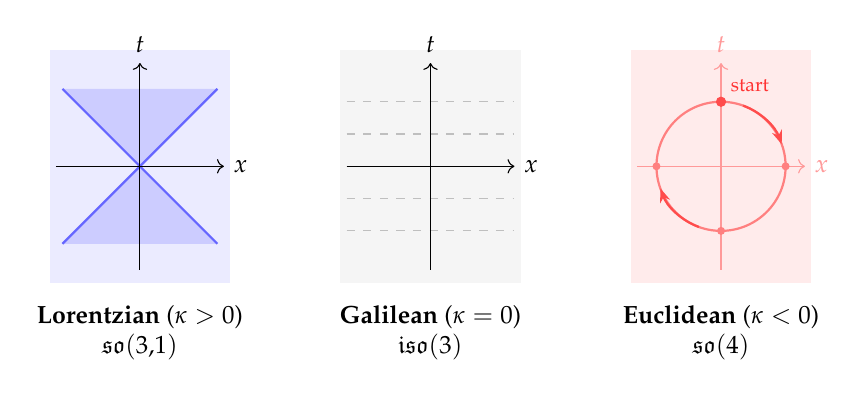
\begin{tikzpicture}[scale=0.82]
  % Lorentzian
  \begin{scope}[shift={(-4.5,0)}]
    \fill[blue!8] (-1.4,-1.8) rectangle (1.4,1.8);
    \fill[blue!20] (0,0) -- (1.2,1.2) -- (-1.2,1.2) -- cycle;
    \fill[blue!20] (0,0) -- (1.2,-1.2) -- (-1.2,-1.2) -- cycle;
    \draw[blue!60, thick] (-1.2,-1.2) -- (0,0) -- (1.2,-1.2);
    \draw[blue!60, thick] (-1.2,1.2) -- (0,0) -- (1.2,1.2);
    \draw[->] (0,-1.6) -- (0,1.6) node[above]{\small $t$};
    \draw[->] (-1.3,0) -- (1.3,0) node[right]{\small $x$};
    \node[below] at (0,-2.0) {\small\textbf{Lorentzian} ($\kappa > 0$)};
    \node[below] at (0,-2.45) {\small $\mathfrak{so}(3{,}1)$};
  \end{scope}
  % Galilean
  \begin{scope}[shift={(0,0)}]
    \fill[gray!8] (-1.4,-1.8) rectangle (1.4,1.8);
    \draw[gray!50, dashed] (-1.3,0) -- (1.3,0);
    \draw[gray!50, dashed] (-1.3,0.5) -- (1.3,0.5);
    \draw[gray!50, dashed] (-1.3,-0.5) -- (1.3,-0.5);
    \draw[gray!50, dashed] (-1.3,1.0) -- (1.3,1.0);
    \draw[gray!50, dashed] (-1.3,-1.0) -- (1.3,-1.0);
    \draw[->] (0,-1.6) -- (0,1.6) node[above]{\small $t$};
    \draw[->] (-1.3,0) -- (1.3,0) node[right]{\small $x$};
    \node[below] at (0,-2.0) {\small\textbf{Galilean} ($\kappa = 0$)};
    \node[below] at (0,-2.45) {\small $\mathfrak{iso}(3)$};
  \end{scope}
  % Euclidean
  \begin{scope}[shift={(4.5,0)}]
    \fill[red!8] (-1.4,-1.8) rectangle (1.4,1.8);
    \draw[->, red!40] (0,-1.6) -- (0,1.6) node[above]{\small $t$};
    \draw[->, red!40] (-1.3,0) -- (1.3,0) node[right]{\small $x$};
    \draw[red!50, thick] (0,0) circle (1.0);
    \draw[-{Stealth[length=5pt]}, red!70, thick] (70:1.0) arc (70:20:1.0);
    \draw[-{Stealth[length=5pt]}, red!70, thick] (250:1.0) arc (250:200:1.0);
    \filldraw[red!70] (0,1.0) circle (2pt) node[above right, font=\scriptsize, red!80] {start};
    \filldraw[red!50] (1.0,0) circle (1.5pt);
    \filldraw[red!50] (0,-1.0) circle (1.5pt);
    \filldraw[red!50] (-1.0,0) circle (1.5pt);
    \node[below] at (0,-2.0) {\small\textbf{Euclidean} ($\kappa < 0$)};
    \node[below] at (0,-2.45) {\small $\mathfrak{so}(4)$};
  \end{scope}
\end{tikzpicture}
\smallskip

{\small\textbf{Figure 1}: The three kinematic universes allowed by the relativity postulate. \textbf{Left}: the Lorentzian case ($\kappa > 0$); the shaded blue region is the set of events accessible within the finite maximum speed, bounded by lightcone lines ($dx/dt = \pm 1/\!\sqrt{\kappa}$). \textbf{Centre}: the Galilean case ($\kappa = 0$); horizontal slices of simultaneity fill all of space. \textbf{Right}: the Euclidean case ($\kappa < 0$); boosts act as rotations, cycling through all directions.}
\end{center}

\smallskip
\noindent\textbf{Lorentzian} ($\kappa > 0$). The transformations are Einstein's. There is a finite maximum speed, and spacetime has lightcones, the V-shaped boundaries shown above, separating events that can influence each other from events that cannot. This is causal structure.

\smallskip
\noindent\textbf{Galilean} ($\kappa = 0$). The transformations are Newton's. Time is universal (the horizontal slices above, where every observer agrees on ``now''), there is no speed limit, and space and time are independent of each other.

\smallskip
\noindent\textbf{Euclidean} ($\kappa < 0$). All four dimensions are equivalent. There is no lightcone, no distinction between past and future. All directions, including time, are geometrically the same. Change your velocity far enough and you loop back to rest.

\medskip
Every treatment since 1910 has agreed that the first postulate alone can't determine the sign of~$\kappa$ \cite{Ignatowski1910,Pauli1921,BerziGorini1969,LevyLeblond1976,Mermin1984,Pal2003,Silagadze2007,Drory2015}. To choose among the three, one must look outside: measure the speed of light, and thereby import Einstein's second postulate or something equivalent. Pauli wrote in 1921: ``Nothing can naturally be said about the sign, magnitude and physical meaning of~[$\kappa$].''

We disagree. The symmetry rules already contain the answer.


\subsection*{Can the rules examine themselves?}

The three universes share the same generators and combination rules. They differ only in the value of~$\kappa$, which controls how strongly the elementary operations interact with each other. Can this internal structure, using only its own resources, distinguish the three cases without any appeal to experiment?

It can. Wilhelm Killing found a way to do this in 1888 \cite{Killing1888}, seventeen years before Einstein's paper. His construction, the Killing form, applies to any set of symmetry rules.

Every set of symmetry rules is built from elementary operations called generators. For the symmetry of motion, there are six: three rotations ($J_1, J_2, J_3$, one for each spatial axis) and three boosts ($K_1, K_2, K_3$, one for each direction of motion). A rotation relates your laboratory to one pointing a different way. A boost relates it to one moving past you, the operation of changing velocity. The relativity postulate is, at bottom, a statement about the boosts.

The rules of the algebra (technically, a Lie algebra, the algebraic structure that encodes continuous symmetries) specify what happens when you perform these operations in sequence, and in particular, when the order matters. Rotations don't commute. Rotate an aeroplane nose-up and then roll it right, and you get a different orientation than if you roll first and pitch second. This sensitivity to ordering is what gives three-dimensional space its rigid geometric structure. Whether the \emph{boosts} share this property depends on~$\kappa$.

Each generator acts as a machine that reshuffles the others. (Mathematicians call this the adjoint action.) When two generators are combined in sequence, the result may mix rotations into boosts and boosts into rotations. The Killing form measures the total reshuffling that each pair produces, formally $B(X,Y) = \mathrm{tr}(\mathrm{ad}_X \circ \mathrm{ad}_Y)$, the trace of the combined reshuffling. It produces a single number, computed entirely from the combination rules. No choices are involved and no external input is needed. Every set of symmetry rules has exactly one Killing form, just as every object has exactly one centre of mass. You compute it; you don't choose it.

For the symmetry rules labelled by~$\kappa$, the result is:
\[
B \;=\; \mathrm{diag}(-4I_3,\;\; 4\kappa\, I_3).
\]
In words: the Killing form registers $-4$ on every rotation and $4\kappa$ on every boost. Rotations always produce a robust, non-zero value, while the boosts produce a value that depends entirely on~$\kappa$.

So we have the self-test. When the Killing form returns a non-zero value for a generator, the algebra ``sees'' that generator and can build geometry from it (the form is non-degenerate on that subspace). When it returns zero, the algebra is blind in that direction and the form degenerates. The value on the boosts now sorts the three universes.


\subsection*{Three verdicts}

\textbf{$\kappa < 0$: No causal structure.}

\smallskip
When $\kappa$ is negative, the Killing form is negative definite: the algebra sees all of its own generators and has no blind spots. But this means the group is compact ($\mathrm{SO}(4)$) and there is no algebraic distinction between spatial and temporal directions. As the diagram above illustrates, the geometry treats all four dimensions of spacetime equivalently. No lightcone, no causal ordering, no way to distinguish past from future. The boosts are periodic: apply enough of them and you return to your starting velocity.

A universe with~$\kappa < 0$ has no notion of cause and effect. Physics, as we understand it, requires one.

\bigskip
\textbf{$\kappa = 0$: The algebra goes blind.}

\smallskip
When $\kappa = 0$, the Killing form returns $4 \times 0 = 0$ on every boost generator. The self-test comes back blank for exactly the operations that the relativity postulate demands: the boosts that connect one inertial frame to another. The rotations still register their full~$-4$. But the boosts are invisible to the algebra's own diagnostic.

The blindness has a concrete consequence. Consider the space of all possible velocities (the coset space $H_\kappa/\mathrm{SO}(3)$, where transformations that differ only by a rotation are treated as the same point, and whose tangent space is spanned by the boosts). Rotational symmetry forces this space to look the same in every direction, so its shape is fixed. (By Schur's lemma, the unique $\mathrm{SO}(3)$-invariant form on the boost subspace is $\delta_{ij}$, up to a positive constant.) But its \emph{scale} is not. How large is a unit of velocity? Is there a natural ruler? That amounts to asking whether there is a special speed built into the geometry, a speed that is the same in all frames and would play the role of~$c$. The Killing form is what should provide the answer: $V = 1/\sqrt{\kappa}$. At $\kappa = 0$, it can't. The shape of the room is known, but the ruler is missing.

\begin{center}
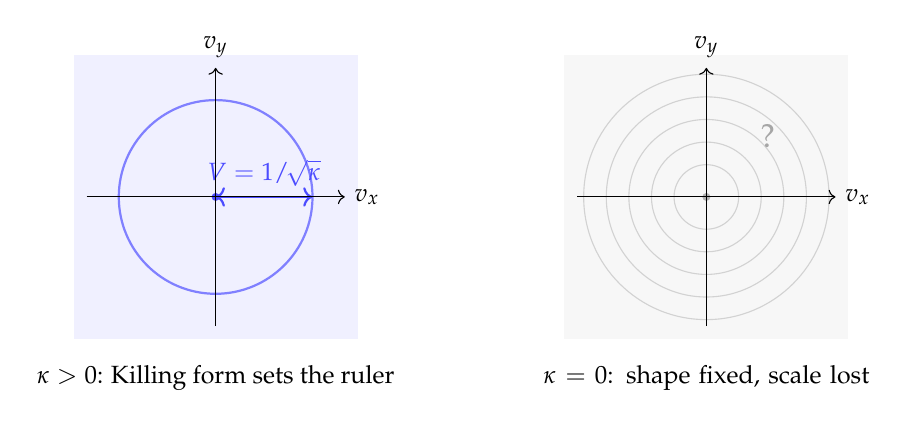
\begin{tikzpicture}[scale=0.82]
  \begin{scope}[shift={(-3.8,0)}]
    \fill[blue!6] (-2.2,-2.2) rectangle (2.2,2.2);
    \draw[blue!50, thick] (0,0) circle (1.5);
    \draw[blue!70, thick, <->] (0,0) -- node[above, font=\small] {$V = 1/\!\sqrt{\kappa}$} (1.5,0);
    \filldraw[blue!70] (0,0) circle (1.5pt);
    \draw[->] (-2.0,0) -- (2.0,0) node[right, font=\small] {$v_x$};
    \draw[->] (0,-2.0) -- (0,2.0) node[above, font=\small] {$v_y$};
    \node[below, font=\small] at (0,-2.45) {\textbf{$\kappa > 0$}: Killing form sets the ruler};
  \end{scope}
  \begin{scope}[shift={(3.8,0)}]
    \fill[gray!6] (-2.2,-2.2) rectangle (2.2,2.2);
    \draw[gray!35] (0,0) circle (0.5);
    \draw[gray!35] (0,0) circle (0.85);
    \draw[gray!35] (0,0) circle (1.2);
    \draw[gray!35] (0,0) circle (1.55);
    \draw[gray!35] (0,0) circle (1.9);
    \filldraw[gray!60] (0,0) circle (1.5pt);
    \draw[->] (-2.0,0) -- (2.0,0) node[right, font=\small] {$v_x$};
    \draw[->] (0,-2.0) -- (0,2.0) node[above, font=\small] {$v_y$};
    \node[font=\large, gray!70] at (0.95,0.95) {?};
    \node[below, font=\small, text width=4.5cm, align=center] at (0,-2.45) {\textbf{$\kappa = 0$}: shape fixed, scale lost};
  \end{scope}
\end{tikzpicture}
\smallskip

{\small\textbf{Figure 2}: Velocity space in the two non-trivial cases. \textbf{Left}: when $\kappa > 0$, the Killing form fixes the radius at $V = 1/\!\sqrt{\kappa}$, giving a definite invariant speed. \textbf{Right}: when $\kappa = 0$, rotational symmetry fixes the shape but no circle is preferred; the scale is undetermined and no invariant speed exists.}
\end{center}

\noindent At $\kappa > 0$ (left), the Killing form fixes the radius of velocity space: there is a definite invariant speed. At $\kappa = 0$ (right), the shape is spherically symmetric (rotational symmetry guarantees that) but every circle is equally valid. The algebra can't choose among them. No invariant speed is determined.

The same failure shows up in spacetime. When $\kappa = 0$, the time equation becomes simply $t' = t$. Time is untouched by the boosts. Every observer in every inertial frame agrees on what time it is. This is Newton's absolute time, a universal clock that ticks the same for everyone. The algebra preserves this structure but doesn't \emph{generate} it. Absolute time is not an approximation, not what relativistic time looks like when things move slowly. It is a fixed point of the Galilean symmetry, something the symmetry leaves entirely alone, hardwired into the $\kappa = 0$ algebra. (The covector $dt$ is invariant under the full homogeneous algebra.) It is a background structure, assumed rather than derived. The spatial geometry must also be supplied from outside.

This is what the relativity postulate was meant to forbid: no preferred frame, no structure put in by hand. But the Galilean algebra, evaluated on its own terms, can't produce the geometry of the universe it describes.

Why does this happen? Because at $\kappa = 0$, the boosts commute ($[K_i, K_j] = 0$): performing boost~$A$ followed by boost~$B$ gives the same result as~$B$ followed by~$A$. Non-commutativity is what gives rotations their geometric rigidity. When the boosts commute, they lose that same rigidity. They can't knit space and time together. The mixing of space and time in Einstein's theory is a direct consequence of the fact that, at $\kappa > 0$, the order of boosts matters ($[K_i, K_j] = -\kappa\,\epsilon_{ijk}\,J_k$, linking boosts back to rotations).

All of these failures trace to this single root: $[K_i, K_j] = 0$. The degenerate Killing form, the missing velocity-space ruler, the decomposition of spacetime into separate time and space sectors, the spacetime metric collapsing to $dt^2$ alone. Galilean mechanics is the low-velocity limit of Lorentzian kinematics, not evidence for an independent framework. And the passage between the two isn't a smooth limit; it is a structural break. The Galilean algebra is a different kind of object from the Lorentzian one.

\bigskip
\textbf{$\kappa > 0$: Everything is determined.}

\smallskip
When $\kappa$ is positive, the Killing form returns $-4$ on the rotations and $4\kappa$ on the boosts. Every generator is visible. No direction is blind.

Velocity space now has a definite geometry, and the ruler is fixed: the Killing form gives $B(K_i, K_j) = 4\kappa\,\delta_{ij}$, which sets the invariant speed at $V = 1/\sqrt{\kappa}$, finite, real, and the same in all frames. Unlike the Galilean case, the scale isn't left dangling. The symmetry rules set it.

Spacetime also acquires a definite geometry, and here the contrast with $\kappa = 0$ is sharpest. At $\kappa = 0$, every observer agrees on time intervals; duration is frame-independent. But at $\kappa > 0$, no observer's time is privileged. Neither time intervals nor spatial distances are frame-independent on their own. The only quantity all observers agree on is the spacetime interval, a single number built from both spatial and temporal separations that combines space and time inseparably. (The invariant metric is $g \propto \mathrm{diag}(1,\, -\kappa,\, -\kappa,\, -\kappa)$, or equivalently $ds^2 = \kappa^{-1}\,dt^2 - dx^2 - dy^2 - dz^2$; the algebra determines this quadratic form uniquely, by Schur's lemma on the irreducible four-dimensional representation.) That is what unification means: the only invariant quantity mixes both.

This geometry has lightcones. Past and future are distinguished. Causal structure exists.

The symmetry rules require no background structure, no absolute time, no spatial ruler from outside, no invariant speed from experiment. They produce everything. The postulate, taken at its word, yields exactly one kind of universe.

\medskip

\begin{center}
\renewcommand{\arraystretch}{1.35}
\begin{tabular}{@{}lccc@{}}
\toprule
& $\kappa < 0$ & $\kappa = 0$ & $\kappa > 0$ \\
\midrule
Killing form on boosts & $4\kappa < 0$ & $0$ & $4\kappa > 0$ \\
Invariant speed $V = 1/\sqrt{\kappa}$ & imaginary & undefined & finite, real \\
Spacetime metric & Euclidean & $dt^2$ only & Lorentzian \\
Causal structure & none & none & lightcones \\
Space--time unification & all alike & impossible & complete \\
Background structure needed & none & yes (time, spatial metric) & none \\
\bottomrule
\end{tabular}
\end{center}


\subsection*{Structure and scale}

A finite invariant speed must exist, and spacetime must be Lorentzian. What the argument doesn't determine is the numerical value of that speed. $V$ depends on~$\kappa$, which sets the conversion factor between units of space and units of time. Measuring $c \approx 3 \times 10^8$\;m/s fixes $\kappa = 1/c^2$. But this is calibration: fitting a number to a framework whose architecture is already determined.

Why does this matter? Because Einstein's second postulate was calibration dressed up as foundation. The symmetry rules themselves demand a finite invariant speed. Experiment tells us \emph{how fast}. The algebra tells us \emph{that}.

Einstein was right that the relativity principle was the deeper of his two postulates, and right that background structure should be eliminated. The tools to finish the job existed in his time. The computation requires nothing beyond the symmetry rules and some straightforward algebra. But the conclusion is the one he reached: there is a finite invariant speed, spacetime is Lorentzian, and space and time are unified.

The speed's value is empirical. Its existence is not.

Einstein needed one postulate, not two.


\begin{thebibliography}{99}
\small

\bibitem{Einstein1905}
A.~Einstein,
``Zur Elektrodynamik bewegter K\"orper,''
\textit{Ann.\ Phys.}\ \textbf{17}, 891 (1905).

\bibitem{Killing1888}
W.~Killing,
``Die Zusammensetzung der stetigen endlichen Transformationsgruppen,''
\textit{Math.\ Ann.}\ \textbf{31}, 252 (1888).

\bibitem{Ignatowski1910}
W.~von Ignatowski,
``Einige allgemeine Bemerkungen \"uber das Relativit\"atsprinzip,''
\textit{Phys.\ Z.}\ \textbf{11}, 972 (1910).

\bibitem{Pauli1921}
W.~Pauli,
\textit{Theory of Relativity},
Teubner, Leipzig (1921); English transl.\ Pergamon (1958).

\bibitem{BacryLL1968}
H.~Bacry and J.-M.~L\'evy-Leblond,
``Possible kinematics,''
\textit{J.\ Math.\ Phys.}\ \textbf{9}, 1605 (1968).

\bibitem{BerziGorini1969}
V.~Berzi and V.~Gorini,
``Reciprocity principle and the Lorentz transformations,''
\textit{J.\ Math.\ Phys.}\ \textbf{10}, 1518 (1969).

\bibitem{LevyLeblond1976}
J.-M.~L\'evy-Leblond,
``One more derivation of the Lorentz transformation,''
\textit{Am.\ J.\ Phys.}\ \textbf{44}, 271 (1976).

\bibitem{Mermin1984}
N.~D.~Mermin,
``Relativity without light,''
\textit{Am.\ J.\ Phys.}\ \textbf{52}, 119 (1984).

\bibitem{Pal2003}
P.~B.~Pal,
``Nothing but relativity,''
\textit{Eur.\ J.\ Phys.}\ \textbf{24}, 315 (2003).

\bibitem{Silagadze2007}
Z.~K.~Silagadze,
``Relativity without tears,''
\textit{Acta Phys.\ Pol.\ B}\ \textbf{39}, 811 (2008).

\bibitem{Drory2015}
A.~Drory,
``The necessity of the second postulate in special relativity,''
\textit{Stud.\ Hist.\ Phil.\ Mod.\ Phys.}\ \textbf{51}, 57 (2015).

\end{thebibliography}

\end{document}
